\documentclass[tikz,border=4pt]{standalone}
\usepackage{pgfplots}\usepgfplotslibrary{groupplots}
\pgfplotsset{compat=1.18}
\definecolor{corba}{HTML}{365FB3}\definecolor{punt}{HTML}{B91C1C}
\begin{document}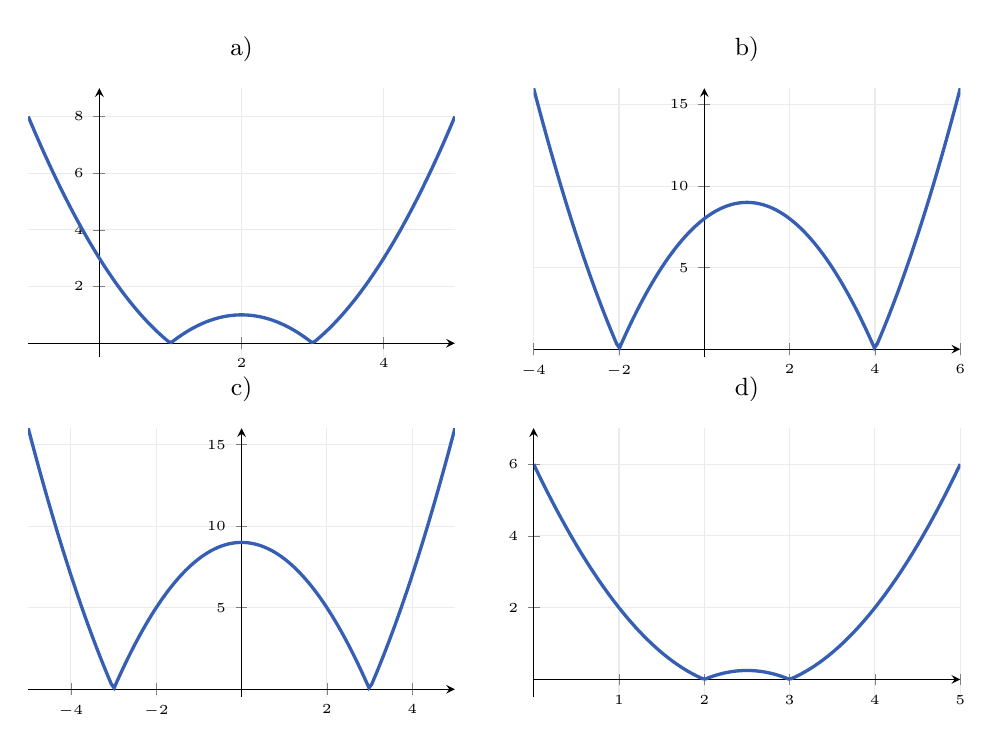
\begin{tikzpicture}
\begin{groupplot}[group style={group size=2 by 2,horizontal sep=1cm,vertical sep=0.9cm},width=7cm,height=5cm,
 axis lines=middle,grid=major,grid style={black!8},tick label style={font=\tiny},title style={font=\small},samples=150]
\nextgroupplot[title={a)},xmin=-1,xmax=5,ymin=-.5,ymax=9]\addplot[corba,very thick,domain=-1:5]{abs(x^2-4*x+3)};
\nextgroupplot[title={b)},xmin=-4,xmax=6,ymin=-.5,ymax=16]\addplot[corba,very thick,domain=-4:6]{abs(-x^2+2*x+8)};
\nextgroupplot[title={c)},xmin=-5,xmax=5,ymin=-.5,ymax=16]\addplot[corba,very thick,domain=-5:5]{abs(x^2-9)};
\nextgroupplot[title={d)},xmin=0,xmax=5,ymin=-.5,ymax=7]\addplot[corba,very thick,domain=0:5]{abs(-x^2+5*x-6)};
\end{groupplot}\end{tikzpicture}\end{document}
